% !TeX engine = xelatex
\documentclass{ctexbeamer}
\usepackage{ctex}
\usepackage{booktabs}
\usepackage{svg}
\usepackage[style=authortitle-comp,backend=bibtex]{biblatex}
\usecolortheme{seagull}
\title{Deep-learning Based Models for Recommender Systems}
\subtitle{Wide \& Deep Learning for Regression/Classification Problems}
\author{Xinyi Li}
\date{\today}
\addbibresource{ref.bib}

\setbeamertemplate{sidebar right}{}
\setbeamertemplate{footline}{%
	\hfill\usebeamertemplate***{navigation symbols}
	\hspace{1cm}\insertframenumber{}/\inserttotalframenumber}
\begin{document}
\begin{frame}
	\titlepage
\end{frame}

\begin{frame}{Overview}
	\tableofcontents
\end{frame}

\begin{frame}{演化图谱\footfullcite{history_graph}}
	\begin{center}
	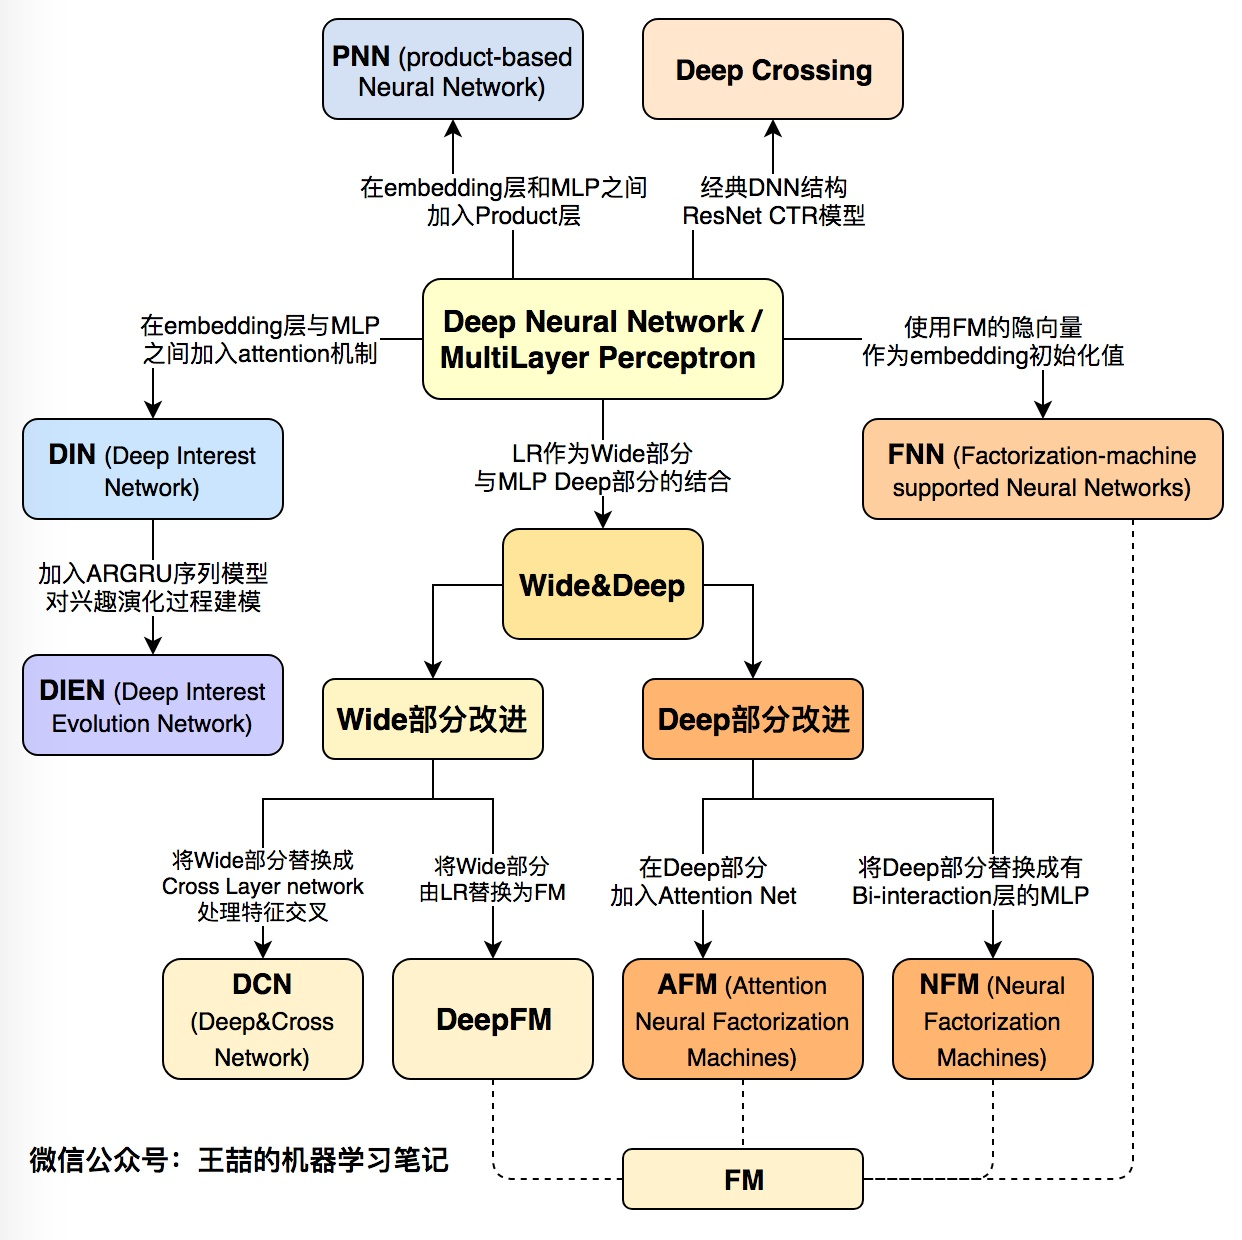
\includegraphics[width=.7\textwidth]{history}
\end{center}
\end{frame}

\section{Deep Cross}
\begin{frame}{Base Model: Deep Crossing \footfullcite{shan2016deep}}
	\framesubtitle{Microsoft}
	\begin{center}
		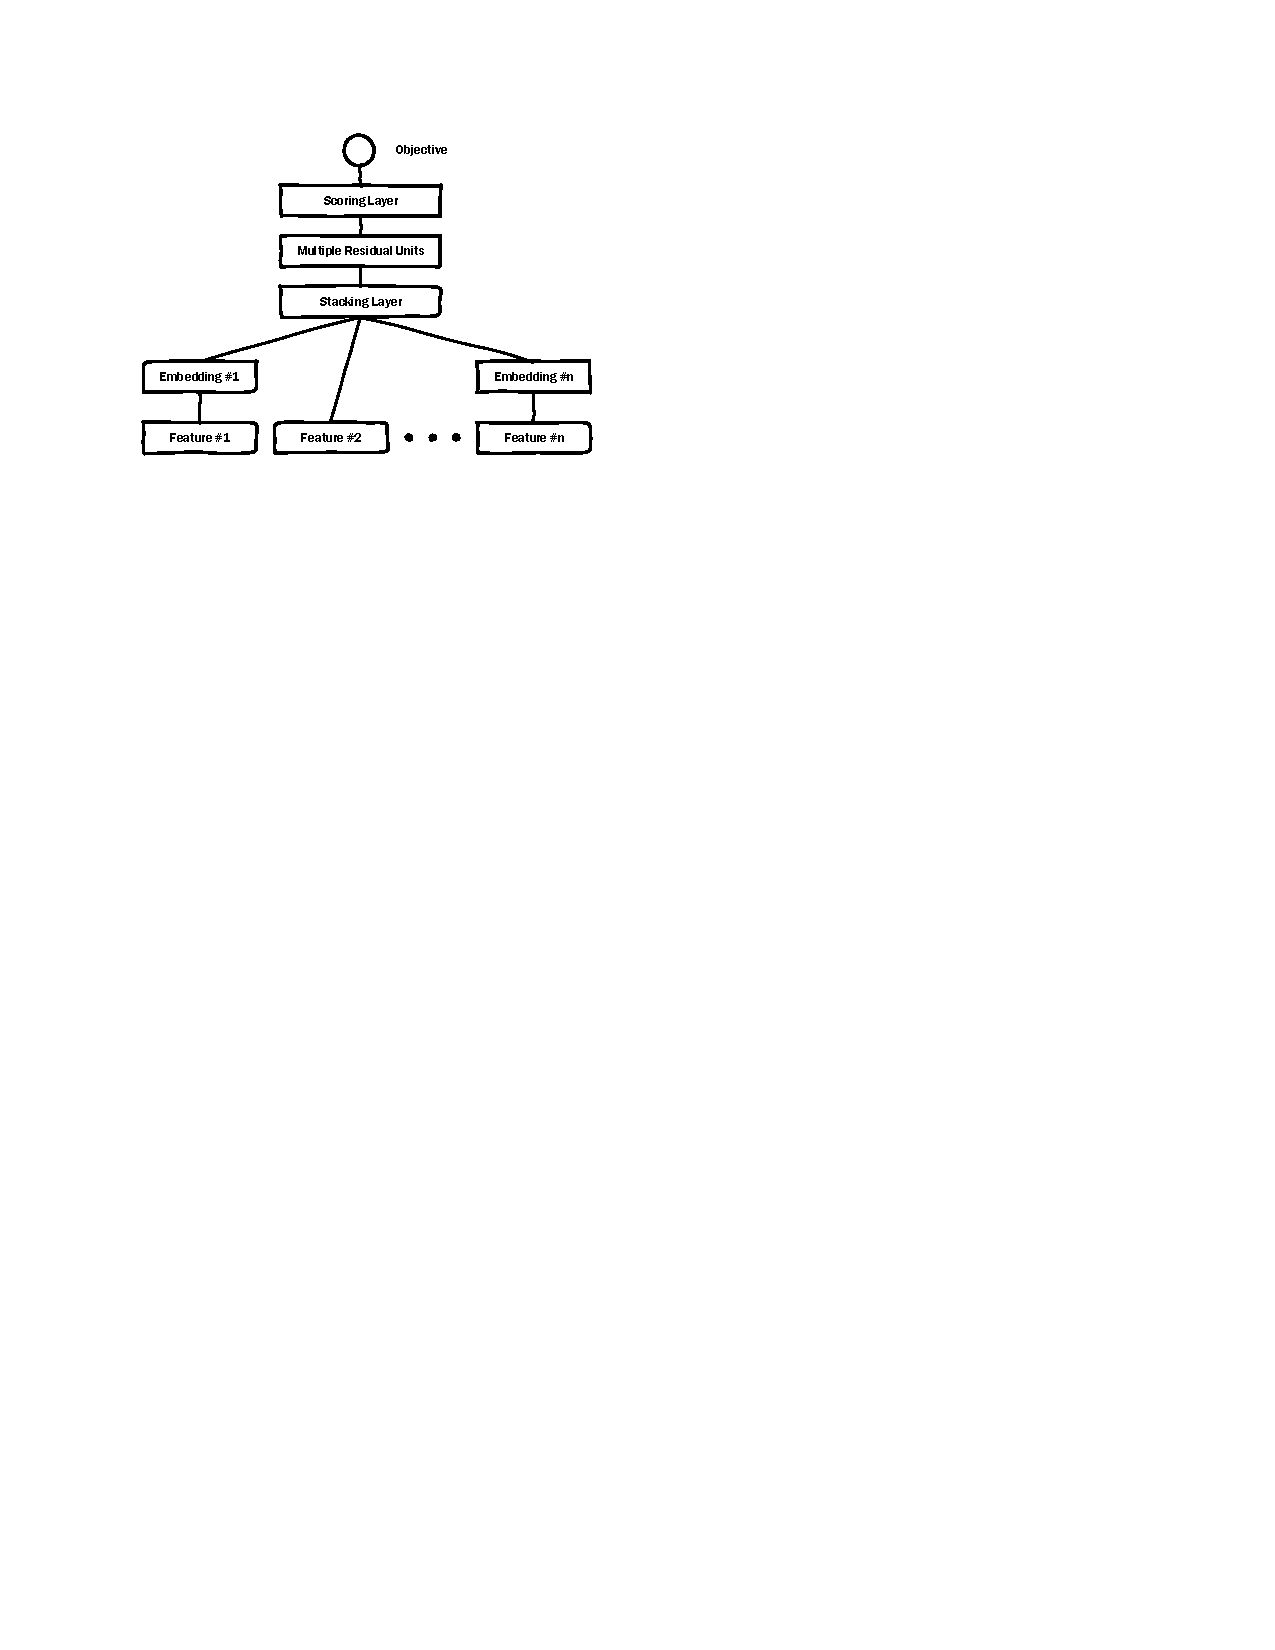
\includegraphics[width=.7\textwidth]{framework/deepcross}
	\end{center}
\end{frame}

\begin{frame}{Deep Crossing}
	\begin{block}{Scoring layer}
		\begin{itemize}
			\item objective: logloss
			\item sigmoid/softmax
		\end{itemize}
	\end{block}
	\begin{block}{Embedding layer}
		高维稀疏特征(id类,one-hot encode) {\color{red}{$\to$}} 低维稠密特征
		$$\mathbf{W}_j: (m_j \times n_j),\quad m_j {\color{red}{<}} n_j$$
		ReLu $$X_j^o = \max (\mathbf{0},\mathbf{W}_j X_j^I + \mathbf{b}_j )$$
	\end{block}
\end{frame}

\begin{frame}{Deep Crossing}
	\begin{block}{Stacking layer}
		concatenate: $X^O = [X_0^O,X_1^O,\cdots,X_K^O]$
	\end{block}
	\begin{block}{{\color{blue}{Residual}} layer}
		2 layers {\color{blue}{ReLu}} transform
		$$X^O = {\color{blue}{\cal F}}(X^I,\{\mathbf{W}_0,\mathbf{W}_1\},\{\mathbf{b}_0,\mathbf{b}_1\})+X^I$$
    \begin{center}
		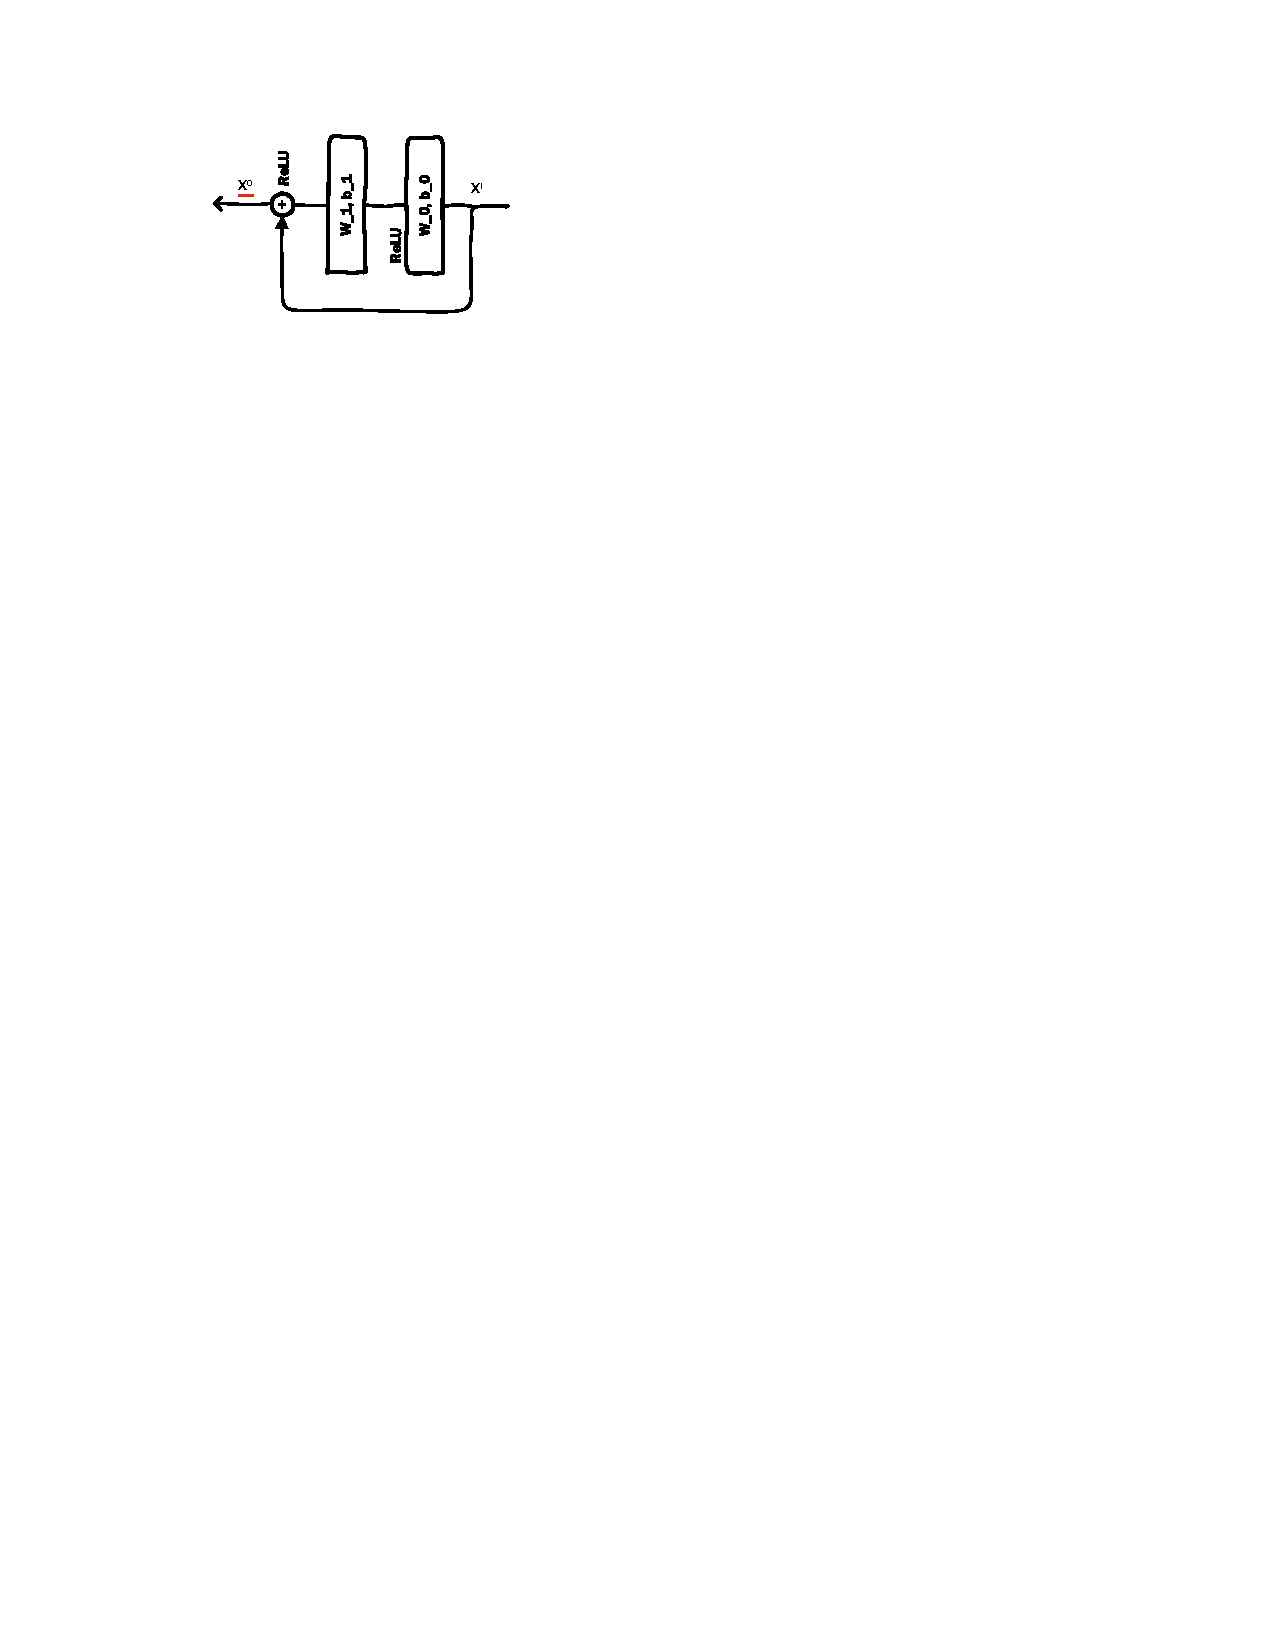
\includegraphics[width=.5\textwidth]{res_unit}
	\end{center}
	\end{block}
\end{frame}

	\section{Factorisation Machine supported Neural Network (FNN)}
\begin{frame}{FNN}
	\framesubtitle{Factorisation Machine supported Neural Network \footfullcite{zhang2016deep}}
	\begin{center}
		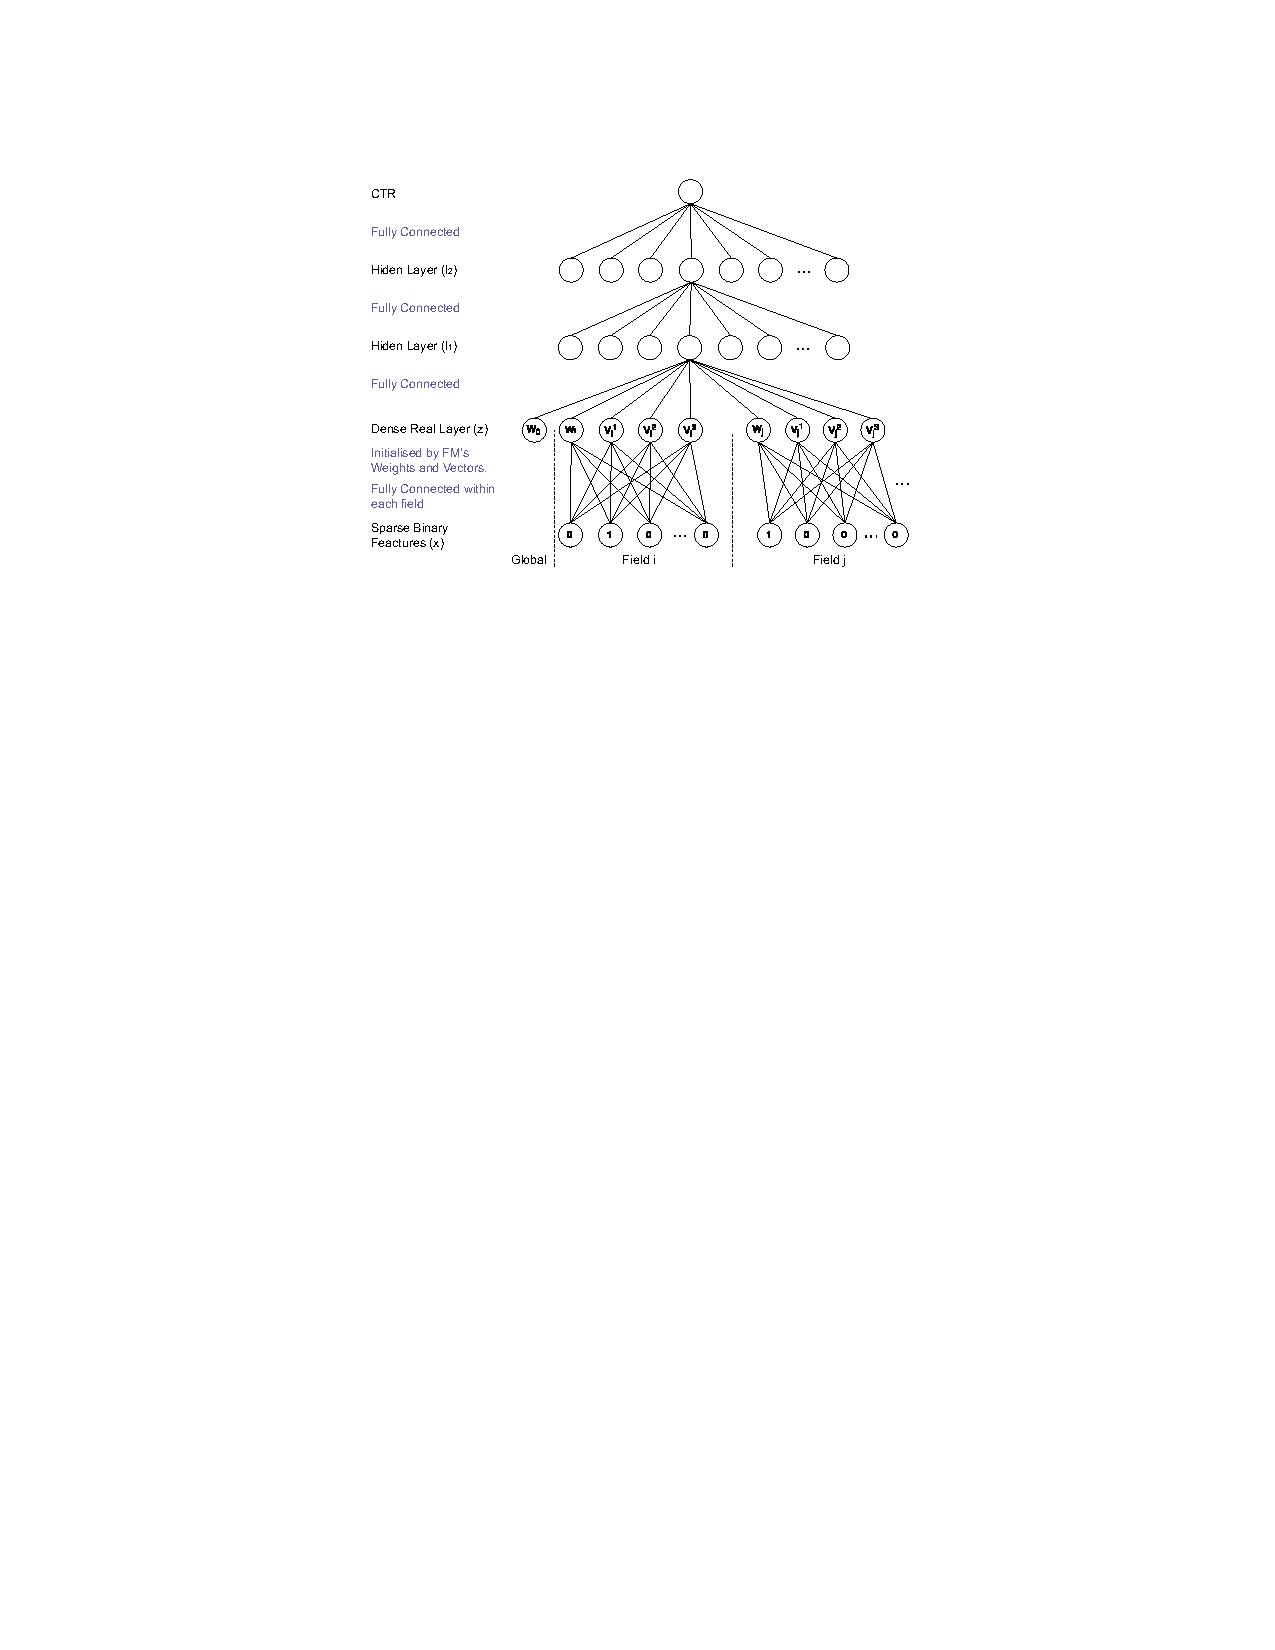
\includegraphics[width=.85\textwidth]{framework/fnn}
	\end{center}
\end{frame}

\begin{frame}{FNN}
	\begin{block}{Hideen layers: $l_1$,$l_2$}
		$l_i = \tanh (\mathbf{W}_i l_{i-1} + \mathbf{b}_i)$
	\end{block}

	\begin{block}{pre-train with FM}
		map 2 features into vectors in a low-rank latent space $\to$ interactions
		$$y \text{FM}({\mathbf{x}}) := sigmoid(w_0 + \sum_{i=1}^{N}{W_i x_i}
		 + \sum_{i=1}^{N}{\sum_{j=i+1}^{N}{<\mathbf{v}_i,\mathbf{v}_j> x_i x_j}})$$
		 $i$-th field
		 $$z_i = \mathbf{W}_0^i \cdot \mathbf{x}[start_i : end_i] = (w_i,v_i^1,v_i^2,\ldots,v_i^K)$$
	$O(end_i - start_i+1) \to O(K+1)$
	\end{block}
\end{frame}

\begin{frame}{FNN}
	\framesubtitle{DeepCTR implement}
	\begin{center}
		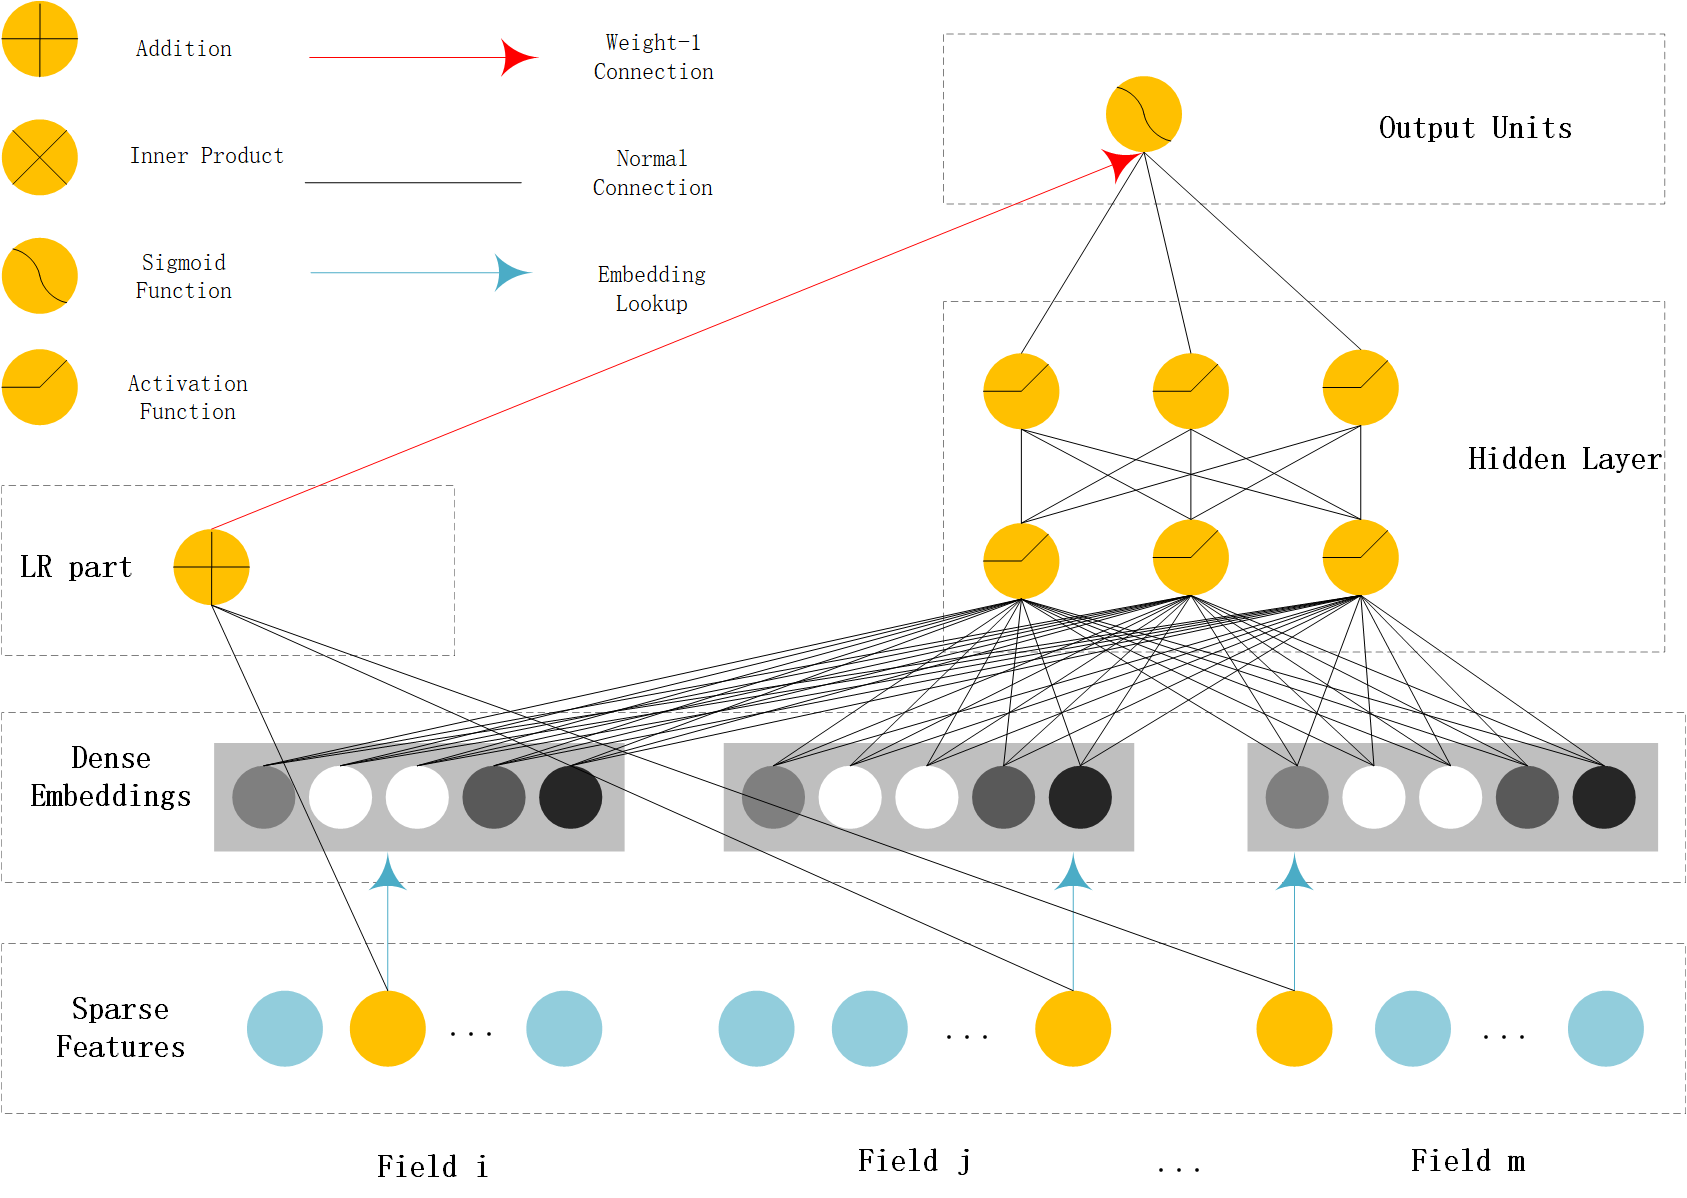
\includegraphics[width=.9\textwidth]{FNN}
	\end{center}
\end{frame}

\section{Product-based Neural Network (PNN)}
\begin{frame}{PNN}
	\framesubtitle{Product-based Neural Network \footfullcite{qu2016product}}
	\begin{center}
		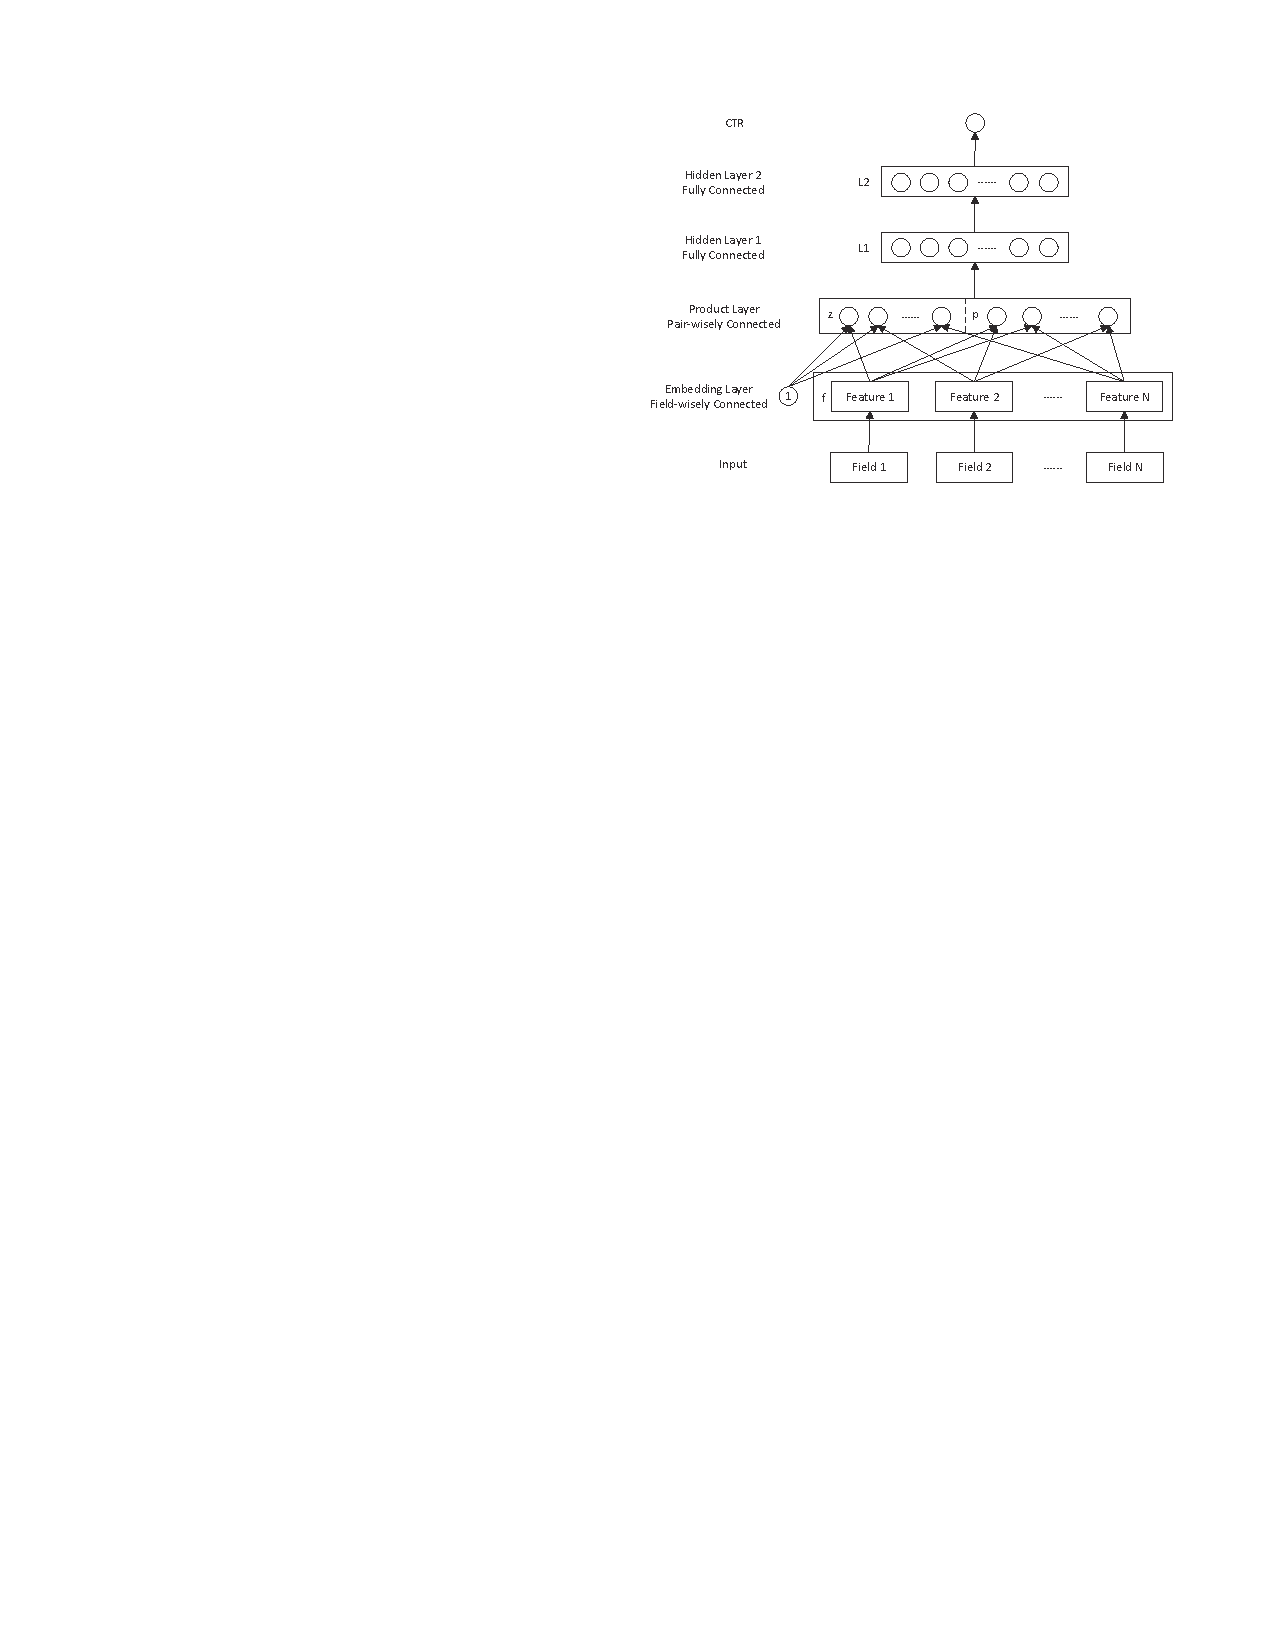
\includegraphics[width=.85\textwidth]{framework/pnn}
	\end{center}
\end{frame}

\section{Wide \& Deep Learning}
\begin{frame}{Wide \& Deep Learning \footfullcite{cheng2016wide}}
\begin{columns}
	\column{.5\textwidth}
	\begin{block}{Wide}
		\begin{itemize}
			\item Memorization(记忆性)
			\item single-layer sparse features (e.g. id)
			\item 记住历史数据的现有关联
		\end{itemize}
	\end{block}
	\column{.5\textwidth}
	\begin{block}{Deep}
		\begin{itemize}
			\item Generalization(泛化性)
			\item Embedding sparse $\to$ dense $\to$ multi-layers DNN
			\item 挖掘数据的潜在关联
		\end{itemize}
	\end{block}
	\end{columns}
	\begin{block}{Binary features $\to$ cross-product transform}
		$\phi (\mathbf{x}) = \prod_{i=1}^{d} {x_i^{c_{ki}}} \quad c_{ki} \in \{0,1\}$
	\end{block}
	\begin{block}{LR}
		Jointly Training: optimizes all parameters (wide \& deep) {\textbf{simultaneously}} (rather than ensemble)
	\end{block}
\end{frame}

\begin{frame}{Wide \& Deep Learning}
	\framesubtitle{Framework for Google Store}
	\begin{center}
		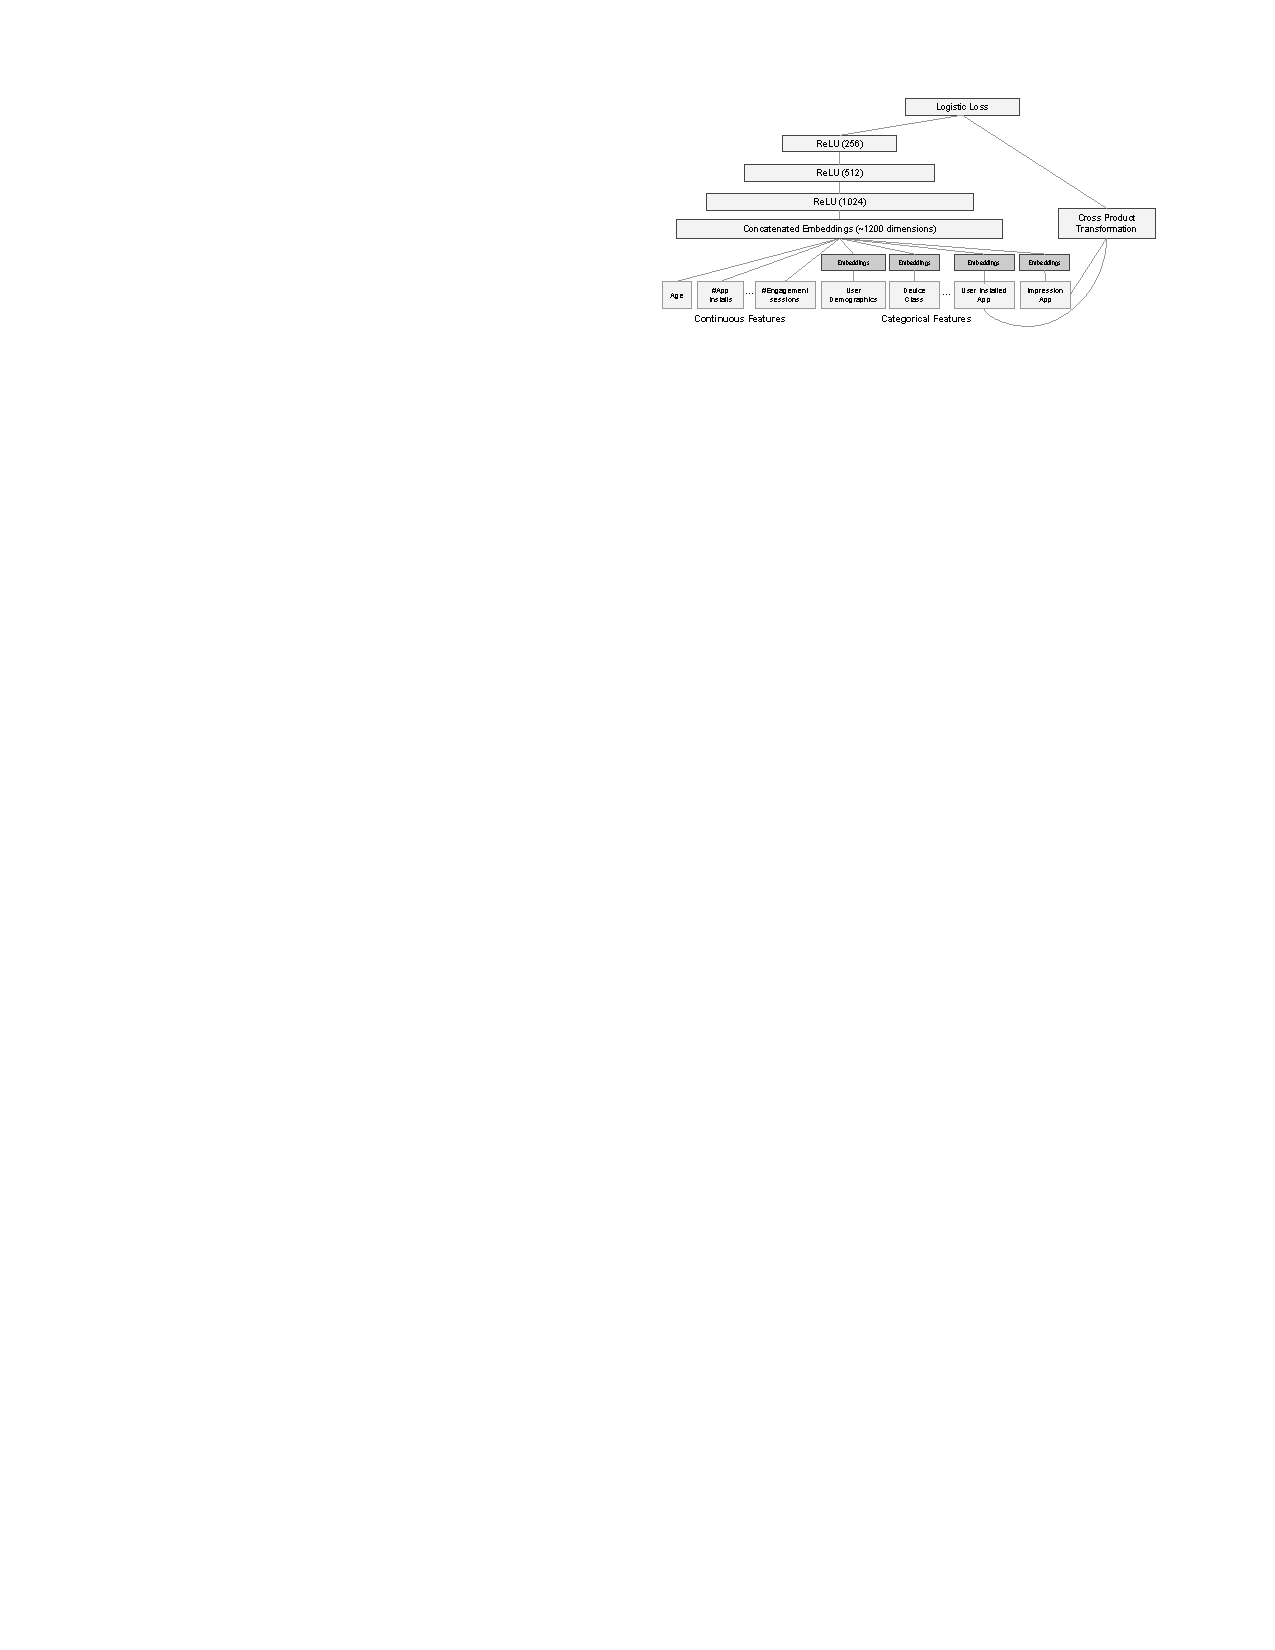
\includegraphics[width=1.1\textwidth]{framework/wdl}
	\end{center}
\end{frame}

\begin{frame}{Wide Part}
	\framesubtitle{Generalized Framework}
	\begin{center}
		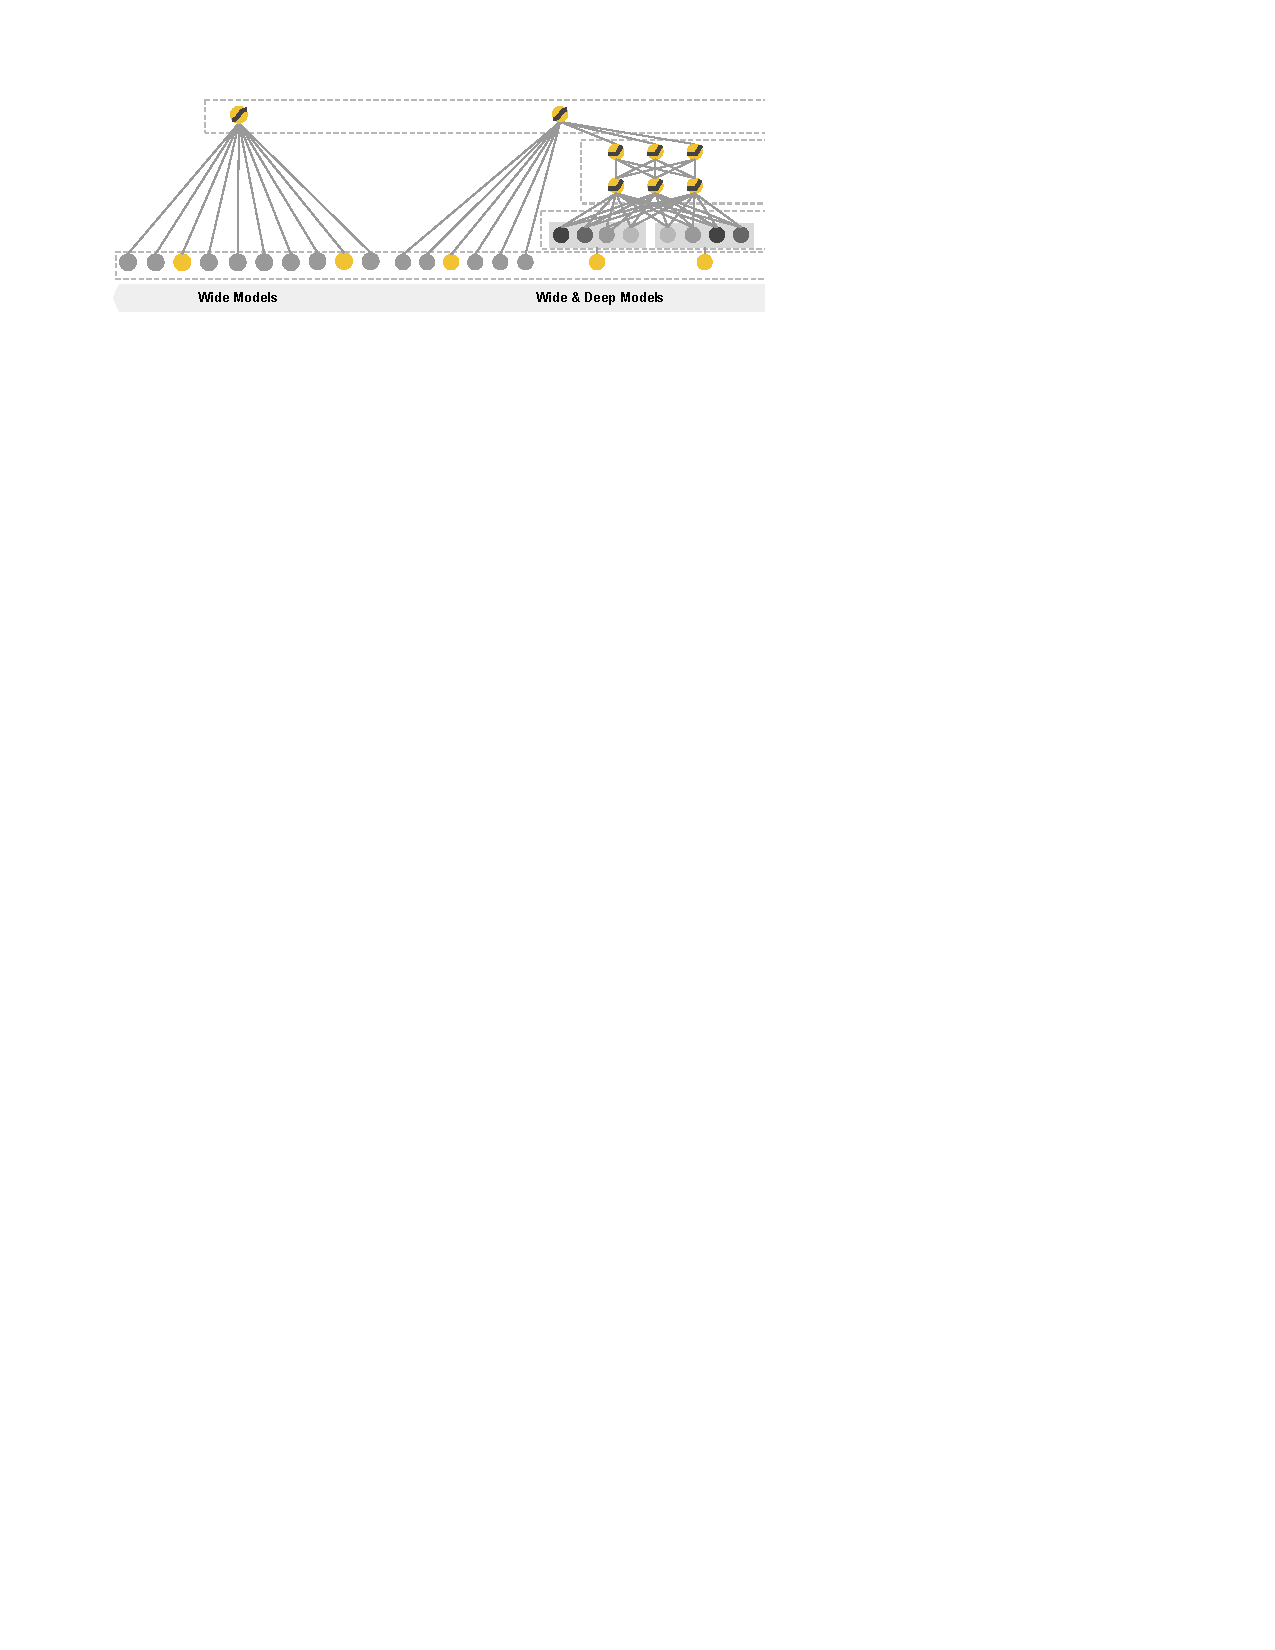
\includegraphics[width=\textwidth]{framework/wide}
	\end{center}
\end{frame}

\begin{frame}{Deep Part}
	\framesubtitle{Generalized Framework}
	\begin{center}
		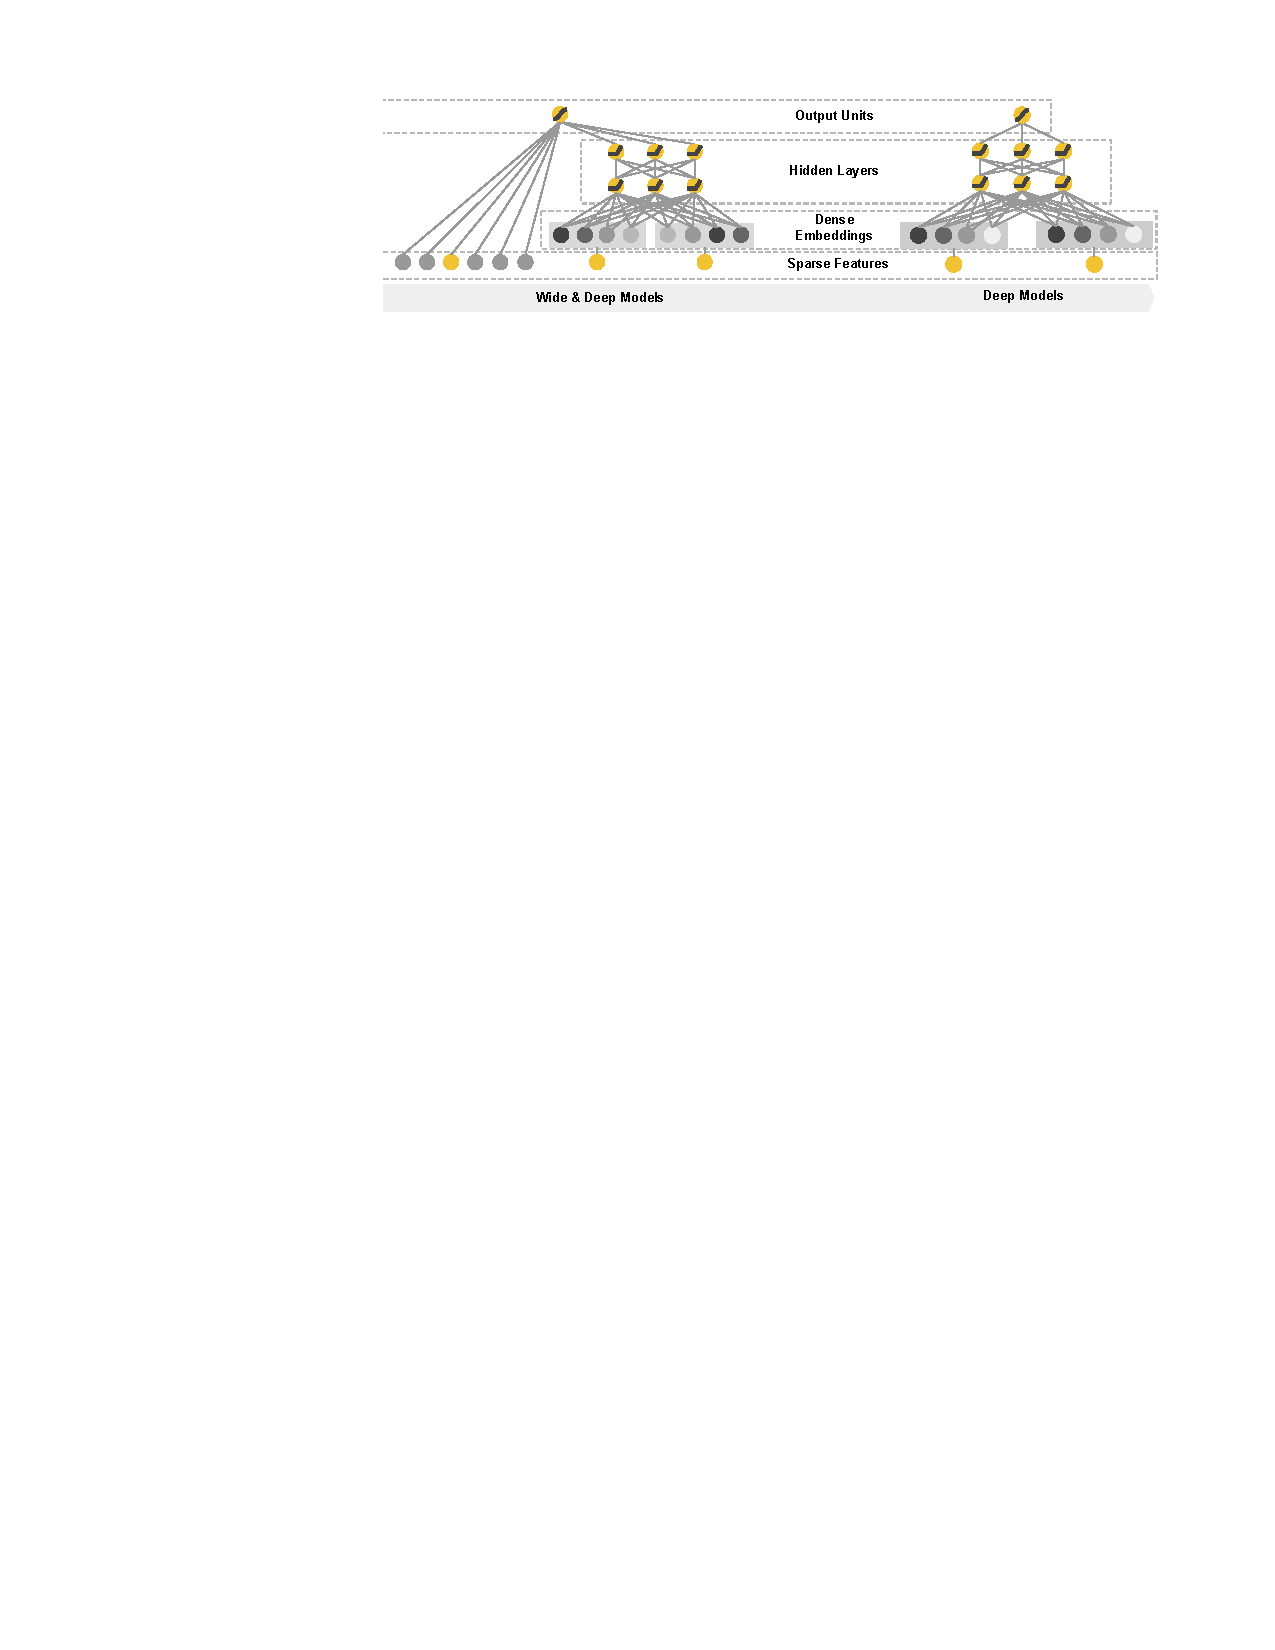
\includegraphics[width=\textwidth]{framework/deep}
	\end{center}
\end{frame}

\section{DeepFM}

\begin{frame}{DeepFM}
	\framesubtitle{Factorization-Machine based Neural Network \footfullcite{guo2017deepfm}}
	\begin{center}
		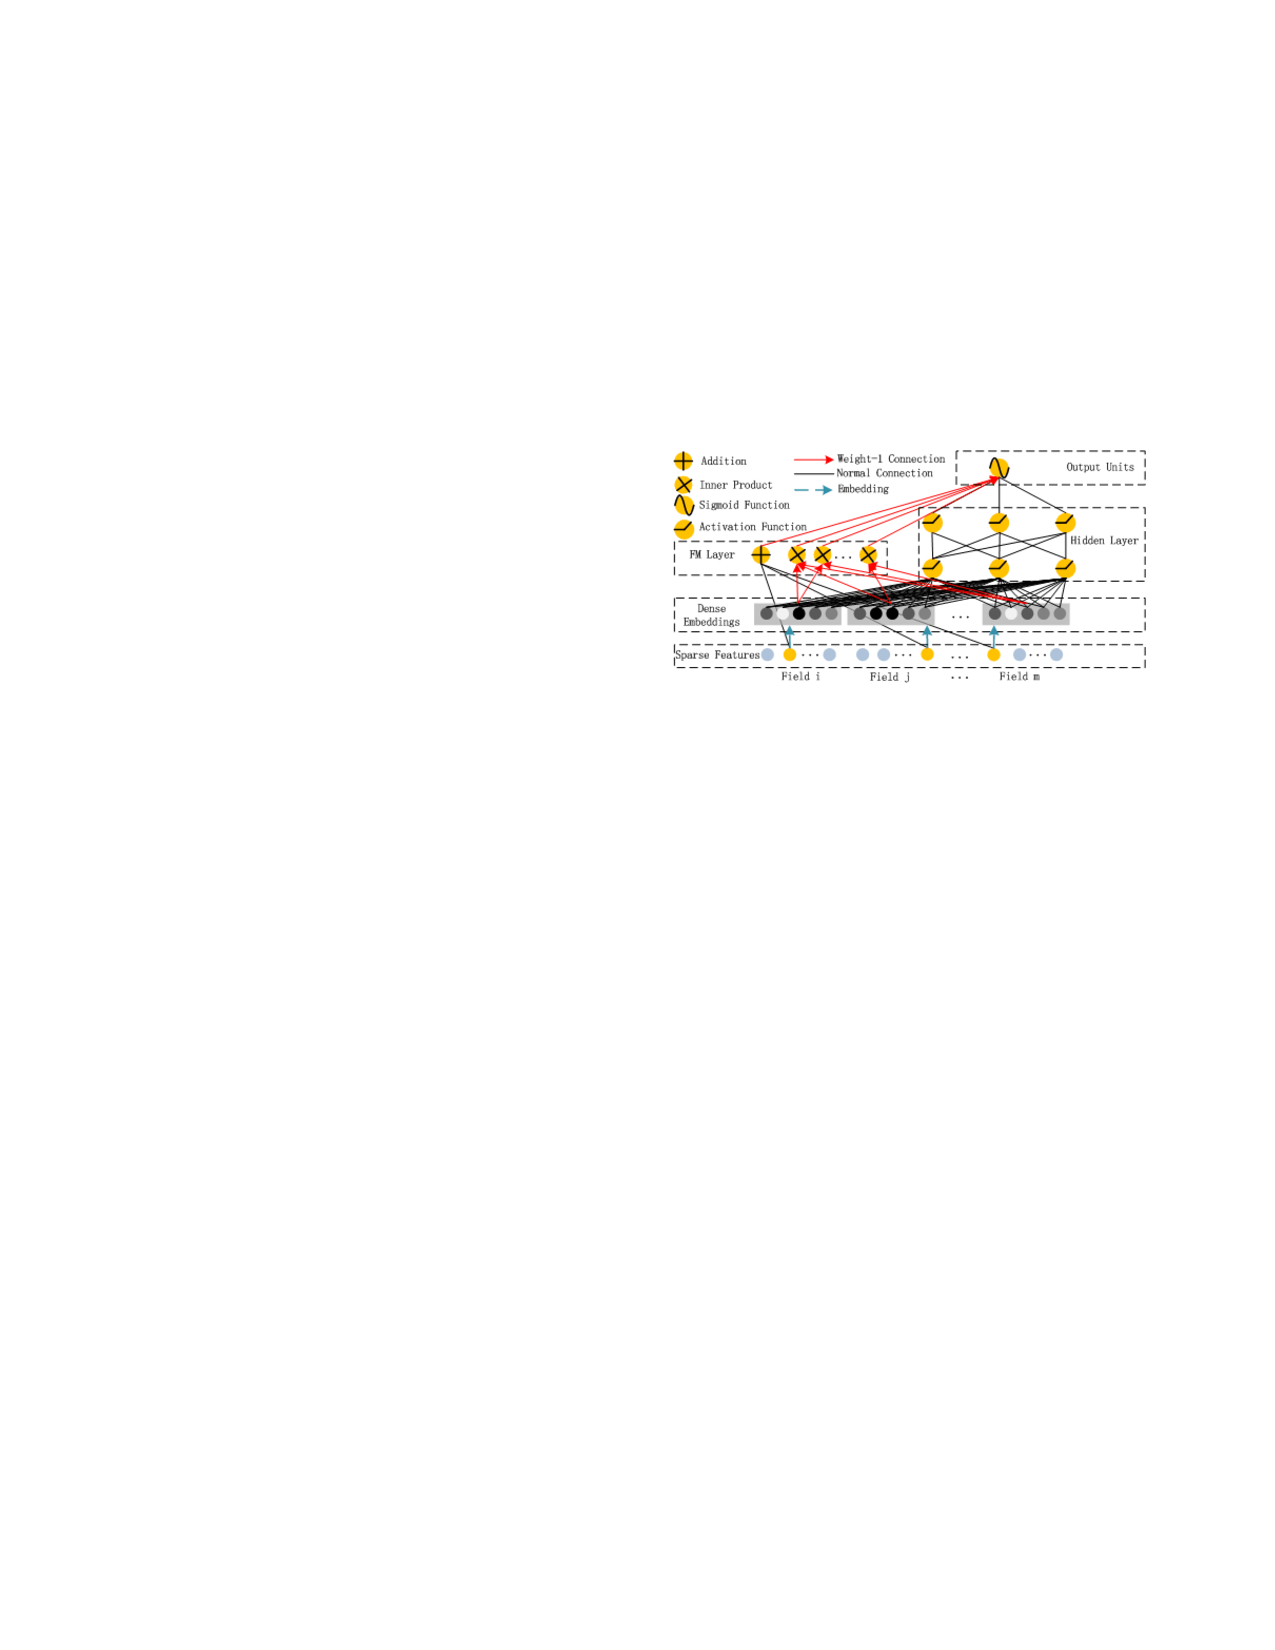
\includegraphics[width=\textwidth]{framework/deepfm}
	\end{center}
\end{frame}

\section{Deep\&Cross Network (DCN)}

\begin{frame}{DCN}
	\framesubtitle{Deep\&Cross Network \footfullcite{wang2017deep}}
	\begin{center}
		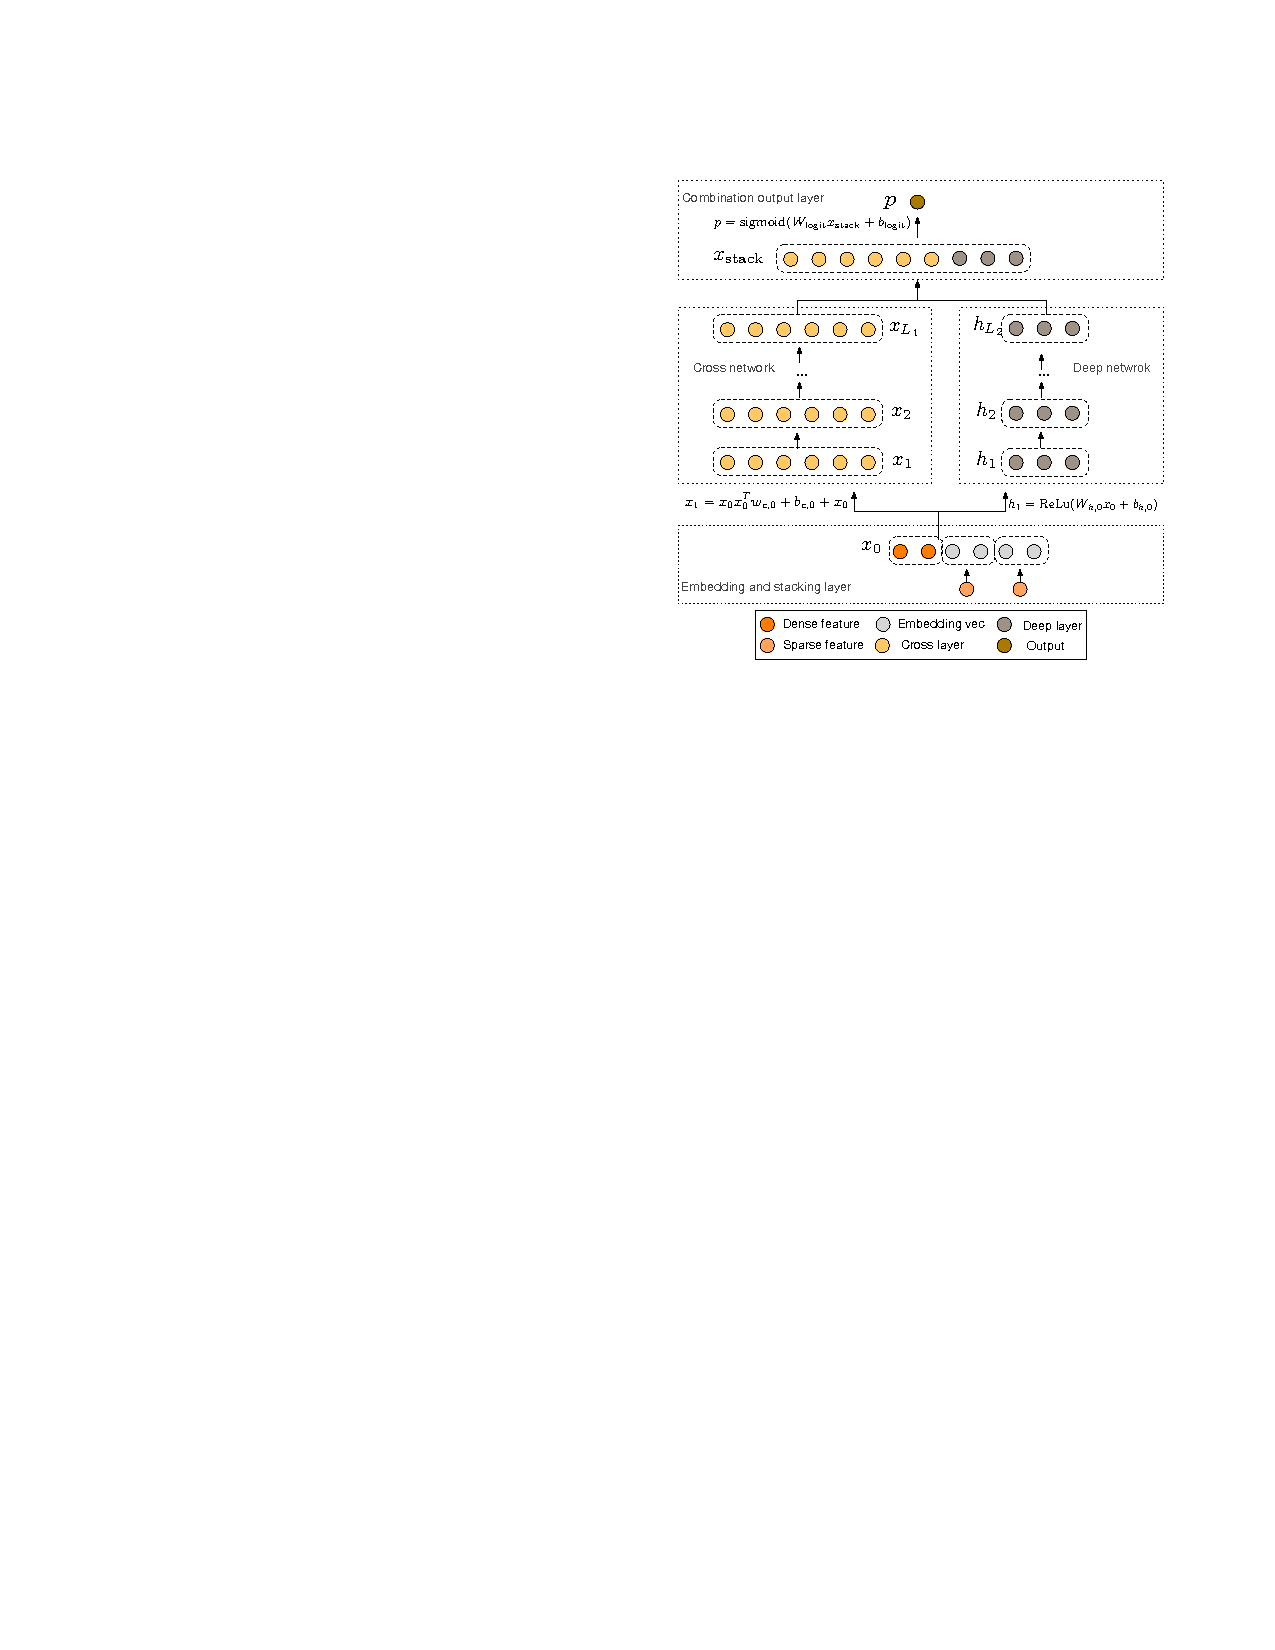
\includegraphics[width=.65\textwidth]{framework/dcn}
	\end{center}
\end{frame}

\section{Attentional Factorization Machines (AFM)}

\begin{frame}{AFM}
	\framesubtitle{Attentional Factorization Machines \footfullcite{xiao2017attentional}}
	\begin{center}
		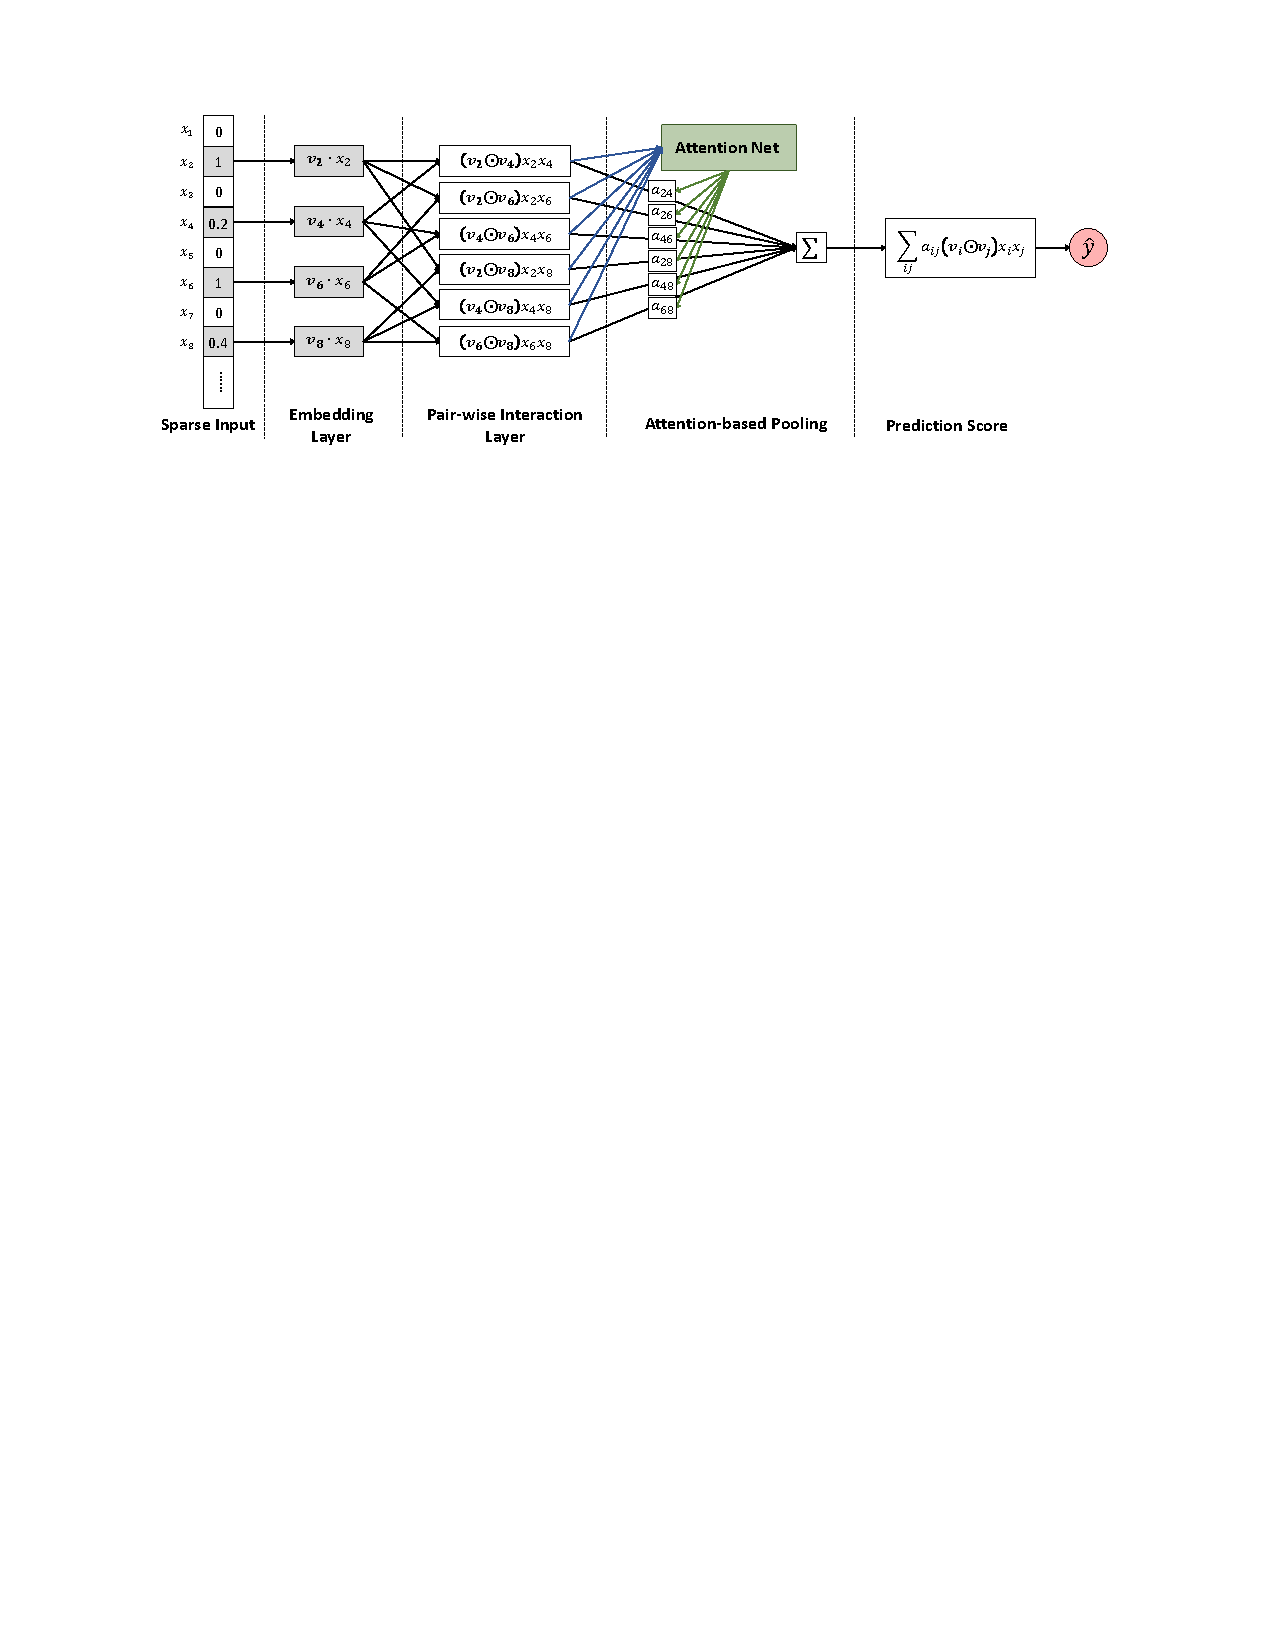
\includegraphics[width=\textwidth]{framework/afm}
	\end{center}

\end{frame}
\section{Implements}
\begin{frame}{Implements}
Demo / Libraries
	\begin{enumerate}
		\item Keras functional API demo: \url{https://github.com/sararob/keras-wine-model}
		\item TensorFlow built-in
		\item \textbf{DeepCTR}: \url{https://github.com/shenweichen/DeepCTR}
	\end{enumerate}
	Practice Tips:
	\begin{enumerate}
		\item Text description features (e.g. address)$\to$ deep part input
		\item Dense dropout
		\item Increase hidden units/layers above embedding layers
		\item ……
	\end{enumerate}
	\centering
	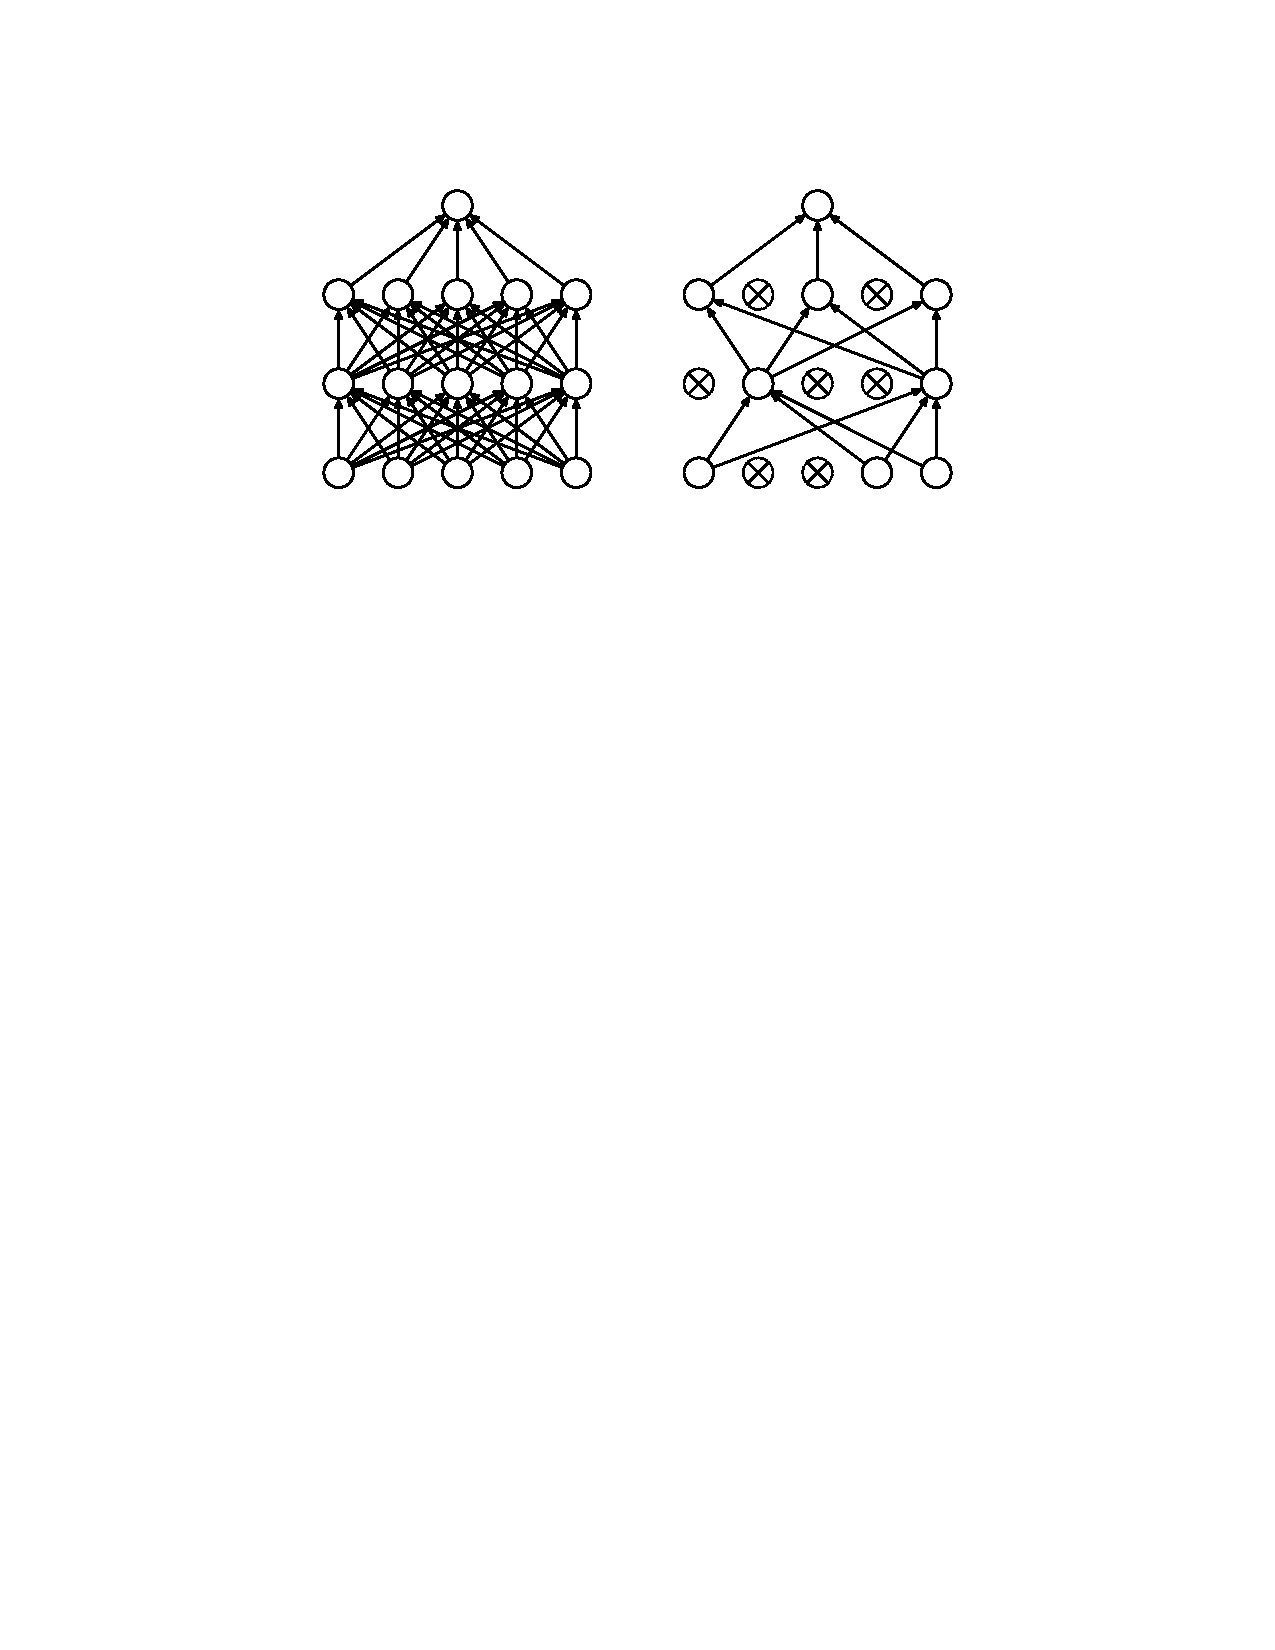
\includegraphics[width=.5\textwidth]{dropout}
\end{frame}

\begin{frame}{}
	\centering
	\Huge{Thanks}
\end{frame}

\end{document}
